\chapter{Đọc thêm 1: Phân rã Giá trị Kỳ dị (SVD) (Murphy)}
\label{ch:M3L4DT1}

% Nguồn: Murphy, K. P. ``Probabilistic Machine Learning: An Introduction.'' MIT Press, 2022, Sections 7.5.1-7.5.2, tr. 259-261.
% Phần cần đọc: Sections 7.5.1 (Basics), 7.5.2 (Connection Between SVD and EVD)
% Nội dung bắt buộc đọc: được kiểm tra trong mọi bài đánh giá (kể cả Quiz).

\section{Thông tin nguồn}

\begin{itemize}
  \item \textbf{Nguồn:} Murphy, Kevin Patrick. \emph{Probabilistic Machine Learning: An Introduction}. MIT Press, 2022. \url{https://probml.github.io/pml-book/book1.html}
  \item \textbf{Phần cần đọc:} Sections 7.5.1-7.5.2 (tr. 259-261)
\end{itemize}

\section{7.5 Phân rã Giá trị Kỳ dị (SVD)}

Bây giờ ta bàn về SVD, phép phân rã tổng quát hóa phân rã giá trị riêng (EVD) cho các ma trận chữ nhật.

\subsection{7.5.1 Cơ bản}

Bất kỳ ma trận (thực) $m \times n$ nào $\mathbf{A}$ đều có thể được phân rã thành

\begin{equation}
\mathbf{A} = \mathbf{U}\mathbf{S}\mathbf{V}^{\mathsf{T}} = \sigma_1 \begin{pmatrix} | \\ \boldsymbol{u}_1 \\ | \end{pmatrix} \begin{pmatrix} - & \boldsymbol{v}_1^{\mathsf{T}} & - \end{pmatrix} + \cdots + \sigma_r \begin{pmatrix} | \\ \boldsymbol{u}_r \\ | \end{pmatrix} \begin{pmatrix} - & \boldsymbol{v}_r^{\mathsf{T}} & - \end{pmatrix}
\tag{7.178}
\end{equation}

trong đó $\mathbf{U}$ là một ma trận $m \times m$ có các cột trực chuẩn (nên $\mathbf{U}^{\mathsf{T}}\mathbf{U} = \mathbf{I}_m$), $\mathbf{V}$ là một ma trận $n \times n$ có các hàng và cột trực chuẩn (nên $\mathbf{V}^{\mathsf{T}}\mathbf{V} = \mathbf{V}\mathbf{V}^{\mathsf{T}} = \mathbf{I}_n$), và $\mathbf{S}$ là một ma trận $m \times n$ chứa $r = \min(m,n)$ \textbf{giá trị kỳ dị} $\sigma_i \geq 0$ nằm trên đường chéo chính, với các phần còn lại được lấp đầy bằng 0. Các cột của $\mathbf{U}$ là các \textbf{vector kỳ dị trái}, và các cột của $\mathbf{V}$ là các vector kỳ dị phải. Phép phân rã này được gọi là \textbf{phân rã giá trị kỳ dị} hay \textbf{SVD} của ma trận. Xem Hình 7.8 để có một ví dụ minh họa.

\begin{figure}[H]
\centering
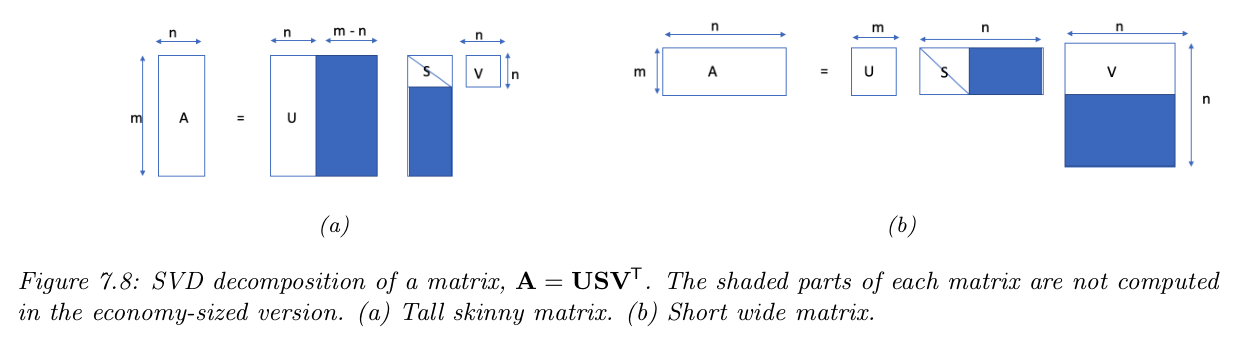
\includegraphics[width=0.85\linewidth]{gfx/m3l4_murphy_fig7-8_svd_decomposition.png}
\par\smallskip{\small \textbf{Hình 7.8:} Phân rã SVD của một ma trận, $\mathbf{A} = \mathbf{U}\mathbf{S}\mathbf{V}^{\mathsf{T}}$. Các phần tô bóng trong mỗi ma trận không được tính trong phiên bản SVD cỡ kinh tế. (a) Ma trận cao gầy. (b) Ma trận rộng thấp.}
\end{figure}

Như có thể thấy từ Hình 7.8a, nếu $m > n$, sẽ có tối đa $n$ giá trị kỳ dị, do đó $m - n$ cột cuối cùng của $\mathbf{U}$ không liên quan (vì chúng sẽ bị nhân với 0). Nếu ta viết ma trận $\mathbf{U}$ dưới dạng $\mathbf{U} = [\mathbf{U}_1, \mathbf{U}_2]$, ta chỉ cần tính $\mathbf{U}_1$. \textbf{SVD cỡ kinh tế} (economy sized SVD), còn gọi là \textbf{thin SVD}, tránh phải tính các phần tử không cần thiết đó. Hình 7.8b cho thấy trường hợp ngược lại, khi $m < n$, trong đó ta biểu diễn $\mathbf{V} = [\mathbf{V}_1; \mathbf{V}_2]$, và chỉ cần tính $\mathbf{V}_1$.

Chi phí tính toán SVD là $O(\min(mn^2, m^2n))$. Bạn đọc có thể tìm chi tiết về cách SVD hoạt động trong các giáo trình đại số tuyến tính chuẩn.

\subsection{7.5.2 Mối liên hệ giữa SVD và EVD}

Nếu $\mathbf{A}$ là thực, đối xứng và xác định dương, thì các giá trị kỳ dị bằng với các giá trị riêng, và các vector kỳ dị trái và phải bằng với các vector riêng (sai khác một dấu):

\begin{equation}
\mathbf{A} = \mathbf{U}\mathbf{S}\mathbf{V}^{\mathsf{T}} = \mathbf{U}\mathbf{S}\mathbf{U}^{\mathsf{T}} = \mathbf{U}\mathbf{S}\mathbf{U}^{-1}
\tag{7.179}
\end{equation}

Tuy nhiên, lưu ý rằng NumPy luôn trả về các giá trị kỳ dị theo thứ tự giảm dần, trong khi các giá trị riêng không nhất thiết được sắp xếp.

Nói chung, đối với một ma trận thực bất kỳ $\mathbf{A}$, nếu $\mathbf{A} = \mathbf{U}\mathbf{S}\mathbf{V}^{\mathsf{T}}$, ta có

\begin{equation}
\mathbf{A}^{\mathsf{T}}\mathbf{A} = \mathbf{V}\mathbf{S}^{\mathsf{T}}\mathbf{U}^{\mathsf{T}}\mathbf{U}\mathbf{S}\mathbf{V}^{\mathsf{T}} = \mathbf{V}(\mathbf{S}^{\mathsf{T}}\mathbf{S})\mathbf{V}^{\mathsf{T}}
\tag{7.180}
\end{equation}

Do đó

\begin{equation}
(\mathbf{A}^{\mathsf{T}}\mathbf{A})\mathbf{V} = \mathbf{V}\mathbf{D}_n
\tag{7.181}
\end{equation}

nên các vector riêng của $\mathbf{A}^{\mathsf{T}}\mathbf{A}$ bằng với $\mathbf{V}$, các vector kỳ dị phải của $\mathbf{A}$, và các giá trị riêng của $\mathbf{A}^{\mathsf{T}}\mathbf{A}$ bằng với $\mathbf{D}_n = \mathbf{S}^{\mathsf{T}}\mathbf{S}$, là một ma trận đường chéo $n \times n$ chứa bình phương các giá trị kỳ dị. Tương tự, ta có

\begin{equation}
\mathbf{A}\mathbf{A}^{\mathsf{T}} = \mathbf{U}\mathbf{S}\mathbf{V}^{\mathsf{T}}\mathbf{V}\mathbf{S}^{\mathsf{T}}\mathbf{U}^{\mathsf{T}} = \mathbf{U}(\mathbf{S}\mathbf{S}^{\mathsf{T}})\mathbf{U}^{\mathsf{T}}
\tag{7.182}
\end{equation}

\begin{equation}
(\mathbf{A}\mathbf{A}^{\mathsf{T}})\mathbf{U} = \mathbf{U}\mathbf{D}_m
\tag{7.183}
\end{equation}

nên các vector riêng của $\mathbf{A}\mathbf{A}^{\mathsf{T}}$ bằng với $\mathbf{U}$, các vector kỳ dị trái của $\mathbf{A}$, và các giá trị riêng của $\mathbf{A}\mathbf{A}^{\mathsf{T}}$ bằng với $\mathbf{D}_m = \mathbf{S}\mathbf{S}^{\mathsf{T}}$, là một ma trận đường chéo $m \times m$ chứa bình phương các giá trị kỳ dị. Tóm lại,

\begin{equation}
\mathbf{U} = \operatorname{evec}(\mathbf{A}\mathbf{A}^{\mathsf{T}}), \quad \mathbf{V} = \operatorname{evec}(\mathbf{A}^{\mathsf{T}}\mathbf{A}), \quad \mathbf{D}_m = \operatorname{eval}(\mathbf{A}\mathbf{A}^{\mathsf{T}}), \quad \mathbf{D}_n = \operatorname{eval}(\mathbf{A}^{\mathsf{T}}\mathbf{A})
\tag{7.184}
\end{equation}

Nếu ta chỉ dùng phần đã tính (khác 0) trong SVD cỡ kinh tế, ta có thể định nghĩa

\begin{equation}
\mathbf{D} = \mathbf{S}^2 = \mathbf{S}^{\mathsf{T}}\mathbf{S} = \mathbf{S}\mathbf{S}^{\mathsf{T}}
\tag{7.185}
\end{equation}

Cũng lưu ý rằng EVD không phải lúc nào cũng tồn tại, ngay cả với $\mathbf{A}$ vuông, trong khi SVD luôn tồn tại.
